\documentclass[11pt]{article}
\usepackage[margin=1in]{geometry}
\usepackage{amsmath,amssymb}
\usepackage{enumerate}
\usepackage{array}
\usepackage{tikz}
\usetikzlibrary{trees}
\usepackage[most]{tcolorbox}
\usepackage{hyperref}
\hypersetup{colorlinks=true,linkcolor=blue!50!black}
\setlength{\parindent}{0pt}
\setlength{\parskip}{5pt}

\tikzset{
  dec/.style={circle,fill,inner sep=1.6pt},
  gametree/.style={level distance=17mm, every node/.style={font=\small}},
  opt/.style={line width=1.6pt}
}

\newtcolorbox{keyidea}[1][Key idea]{colback=blue!4,colframe=blue!45!black,fonttitle=\bfseries,title={#1},breakable}
\newtcolorbox{pitfall}[1][Common mistakes]{colback=red!4,colframe=red!50!black,fonttitle=\bfseries,title={#1},breakable}
\newtcolorbox{selfcheck}[1][Check yourself]{colback=green!4,colframe=green!40!black,fonttitle=\bfseries,title={#1},breakable}

\newcommand{\BR}{\mathrm{BR}}

\title{Problem set 2 \\ \large Learning Guide: walkthrough and explanations}
\author{Econ 5030}
\date{Due 10/12/26}

\begin{document}
\maketitle

\begin{center}
\begin{minipage}{0.88\textwidth}
\small
\textbf{How to use this guide.} Part 0 builds every tool the problem set needs, starting from scratch: what a game is, strategies versus actions, normal and extensive forms, dominance, Nash equilibrium, mixed strategies, and subgame perfection. Parts 1--5 then work through each problem in the order you would solve it on an exam, explaining why each step works, where students usually go wrong, and with a few self-check questions. The separate \emph{Solution Key} contains only what to hand in.
\end{minipage}
\end{center}

\tableofcontents
\newpage

%%%%%%%%%%%%%%%%%%%%%%%%%%%%%%%%%%%%%%%%%%%%%%%%%%%%%%%%%%%%%%%%%%%%%%%
\section*{Part 0. The toolkit}
\addcontentsline{toc}{section}{Part 0. The toolkit}

\subsection*{0.1 What is a game?}
\addcontentsline{toc}{subsection}{0.1 What is a game?}
A \emph{game} is any situation where your payoff depends on what others do as well as on what you do. To describe a game completely you need:
\begin{enumerate}
\item \textbf{Players}: who decides.
\item \textbf{Actions and timing}: what each player can physically do, and when.
\item \textbf{Information}: what each player knows about earlier moves at the moment she moves.
\item \textbf{Payoffs}: how much each player likes each possible final outcome.
\end{enumerate}
There are two standard ways to write this down: the \emph{extensive form} (a game tree) and the \emph{normal form} (a matrix). This problem set is mostly about moving between the two.

\subsection*{0.2 The extensive form: game trees}
\addcontentsline{toc}{subsection}{0.2 The extensive form: game trees}
A game tree is read from the top down.
\begin{itemize}
\item Each \textbf{decision node} (dot) is labelled with the player who moves there.
\item Each \textbf{branch} leaving a node is one action available at that node.
\item Each \textbf{terminal node} (end of a path) lists the payoffs, conventionally $(u_1,u_2)$.
\item An \textbf{information set} groups the nodes a player \emph{cannot tell apart} when she moves, and is drawn as a dashed line joining them. If Player 2 does not see Player 1's move, her two nodes are joined: she knows she is at one of them but not which. If she does see the move, each node is its own information set.
\end{itemize}

\begin{center}
\begin{tabular}{cc}
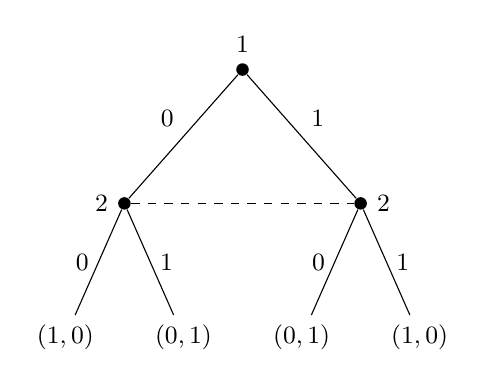
\begin{tikzpicture}[gametree,
  level 1/.style={sibling distance=30mm},
  level 2/.style={sibling distance=15mm}]
\node[dec,label=above:{1}] {}
  child { node[dec,label=left:{2}] (A) {}
    child { node {$(1,0)$} edge from parent node[left] {$0$} }
    child { node {$(0,1)$} edge from parent node[right] {$1$} }
    edge from parent node[above left] {$0$} }
  child { node[dec,label=right:{2}] (B) {}
    child { node {$(0,1)$} edge from parent node[left] {$0$} }
    child { node {$(1,0)$} edge from parent node[right] {$1$} }
    edge from parent node[above right] {$1$} };
\draw[dashed] (A) -- (B);
\end{tikzpicture}
&
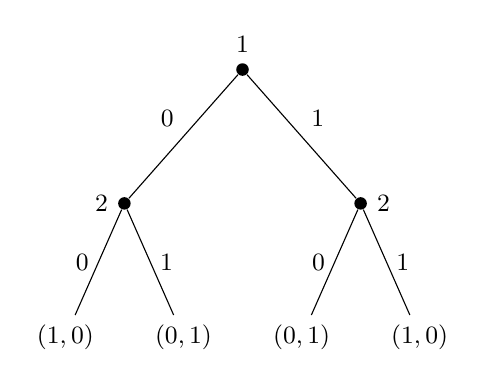
\begin{tikzpicture}[gametree,
  level 1/.style={sibling distance=30mm},
  level 2/.style={sibling distance=15mm}]
\node[dec,label=above:{1}] {}
  child { node[dec,label=left:{2}] {}
    child { node {$(1,0)$} edge from parent node[left] {$0$} }
    child { node {$(0,1)$} edge from parent node[right] {$1$} }
    edge from parent node[above left] {$0$} }
  child { node[dec,label=right:{2}] {}
    child { node {$(0,1)$} edge from parent node[left] {$0$} }
    child { node {$(1,0)$} edge from parent node[right] {$1$} }
    edge from parent node[above right] {$1$} };
\end{tikzpicture}
\\
\small (a) Player 2 does \emph{not} observe Player 1 & \small (b) Player 2 \emph{does} observe Player 1 \\
\small (simultaneous; one information set) & \small (sequential; two information sets)
\end{tabular}
\end{center}
These are the two games in Problem 3. The trees look almost identical; the only difference is the dashed line, and that one line changes the strategy sets.

\subsection*{0.3 Strategies are complete contingent plans}
\addcontentsline{toc}{subsection}{0.3 Strategies are complete contingent plans}
This is the most important idea in the problem set.

\begin{keyidea}[Strategy]
A \textbf{strategy} for player $i$ specifies an action at \emph{every} information set where $i$ moves, \emph{including information sets that will never be reached} given what the others do. Think of it as instructions you could give a robot playing on your behalf: the robot must know what to do in every situation that could come up.
\end{keyidea}

\textbf{Counting rule.} If player $i$ has information sets $h_1,\dots,h_K$ with $m_1,\dots,m_K$ actions available, then
\[
|S_i| = m_1\times m_2\times\cdots\times m_K .
\]
\begin{itemize}
\item In tree (a), Player 2 has one information set with 2 actions, so $|S_2|=2$.
\item In tree (b), Player 2 has two information sets with 2 actions each, so $|S_2|=2\times2=4$.
\item In Problem 2, Player 2 has 2 information sets with 3 actions each, so $|S_2|=9$.
\item In Problem 5, Player 2 has 3 information sets with 2 actions each, so $|S_2|=8$.
\end{itemize}
\textbf{Notation.} Write a second mover's strategy as a list ordered by the first mover's actions. For example, in Problem 2, $d_2c_2$ means ``play $d_2$ if Player 1 chose $a_1$, play $c_2$ if Player 1 chose $b_1$''. Always state your ordering convention explicitly.

\subsection*{0.4 The normal form}
\addcontentsline{toc}{subsection}{0.4 The normal form}
\begin{keyidea}[Normal form (course notes, Def. 3.1)]
$G=(N,\{S_i\}_{i\in N},\{u_i\}_{i\in N})$: a set of players $N$, a strategy set $S_i$ for each player, and payoff functions $u_i:S\to\mathbb{R}$ defined on strategy profiles $s=(s_1,\dots,s_n)\in S=\prod_j S_j$.
\end{keyidea}
\textbf{How to build it from a tree.}
\begin{enumerate}
\item List every strategy for every player using the counting rule.
\item Make a matrix with one row per Player 1 strategy and one column per Player 2 strategy.
\item For each cell, trace the path through the tree that the two strategies produce, and write down the terminal payoffs. In a sequential game, the second mover's strategy is a list; Player 1's choice selects which entry of the list is actually used.
\end{enumerate}
In the normal form everyone is pictured as choosing a whole strategy at once, before play starts. The order of moves has not disappeared, though. It is built into the strategy sets: a later mover has more strategies because she can condition on what she sees.

\subsection*{0.5 Payoffs are utilities, not money}
\addcontentsline{toc}{subsection}{0.5 Payoffs are utilities, not money}
The numbers in a game represent \emph{preferences} over outcomes. If an outcome gives someone \$30 and their partner \$10, the payoff is how much the person \emph{values} that outcome, which could depend on fairness, guilt, altruism, spite, and so on (course notes, Example~3.4). In pure-strategy analysis payoffs are \emph{ordinal}: any strictly increasing transformation $f_i\circ u_i$ gives the same best responses and equilibria. Once probabilities are involved (beliefs or mixed strategies), payoffs must be von Neumann--Morgenstern utilities, which are unique only up to $a_iu_i+b_i$ with $a_i>0$. Problem 4 is built around this point.

\subsection*{0.6 Best responses and the underlining method}
\addcontentsline{toc}{subsection}{0.6 Best responses and the underlining method}
$\BR_i(s_{-i})=\arg\max_{s_i\in S_i}u_i(s_i,s_{-i})$: the strategies that do best for $i$ \emph{given} what the others do.

\textbf{Underlining method} for a two-player matrix:
\begin{enumerate}
\item For each \emph{column}, underline the row player's \emph{largest first number} (underline all of them if there is a tie).
\item For each \emph{row}, underline the column player's \emph{largest second number} (again, all ties).
\item Every cell with \emph{both} numbers underlined is a pure-strategy Nash equilibrium.
\end{enumerate}
This method is mechanical and it does not miss equilibria. Use it on every matrix.

\subsection*{0.7 Dominance and iterated deletion}
\addcontentsline{toc}{subsection}{0.7 Dominance and iterated deletion}
\begin{keyidea}[Strict vs.\ weak dominance]
$s_i$ is \textbf{strictly dominated} by $s_i'$ if $u_i(s_i',s_{-i})>u_i(s_i,s_{-i})$ for \emph{every} $s_{-i}$: strictly better against everything.\\
$s_i$ is \textbf{weakly dominated} by $s_i'$ if $u_i(s_i',s_{-i})\ge u_i(s_i,s_{-i})$ for every $s_{-i}$, with strict inequality for at least one: never worse and sometimes better.
\end{keyidea}
\textbf{Why delete strictly dominated strategies?} A rational player never uses one: whatever she believes about the others, switching to the dominating strategy pays strictly more.

\textbf{Why iterate?} After round 1, if I know you are rational, I know you won't play your dominated strategies. Then I can compare my strategies only against what remains, and some of my strategies may now be dominated. Each round adds one more layer of ``I know that you know that I am rational'' (course notes, Sec.~3.5).

\textbf{Procedure (IDSDS).}
\begin{enumerate}
\item For each player, compare every pair of remaining strategies cell by cell against all remaining opponent strategies.
\item Delete every strictly dominated strategy (for all players in the same round is fine).
\item Repeat on the smaller game until nothing more can be deleted. What survives is the \emph{solution set}.
\end{enumerate}
For strict dominance in finite games the \textbf{order of deletion does not matter}: you end up with the same survivors. With weak dominance, the order can change the answer, which is why the problem asks for strict dominance.

A strategy can be strictly dominated by a \emph{mixed} strategy even when no pure strategy dominates it. You do not need that refinement in this problem set, because every deletion here is by a pure strategy.

\subsection*{0.8 Nash equilibrium}
\addcontentsline{toc}{subsection}{0.8 Nash equilibrium}
\begin{keyidea}[Nash equilibrium (course notes, Def. 3.19)]
A profile $s^*$ is a Nash equilibrium if $s_i^*\in\BR_i(s^*_{-i})$ for every $i$: no player can gain by changing her own strategy while the others keep theirs.
\end{keyidea}
\textbf{How to check a candidate.} Fix the others' strategies and ask whether this player can do strictly better by switching. Do this for each player. If no player can, the candidate is an equilibrium.

\textbf{Relationship to dominance.}
\begin{itemize}
\item A strictly dominated strategy is never part of a Nash equilibrium (Prop.~3.23). More generally, anything removed by IDSDS gets probability zero in every equilibrium, pure or mixed.
\item So if IDSDS leaves a single profile, that profile is the \emph{unique} Nash equilibrium, including mixed equilibria. This is the fast route in Problems 1 and 4.
\end{itemize}

\textbf{Mixed strategies and the indifference principle.} A mixed strategy $\sigma_i$ is a probability distribution over $S_i$. In a mixed equilibrium, \emph{every pure strategy played with positive probability must give the same, maximal expected payoff} (support property, Prop.~3.34). So to find a mixed equilibrium you choose each player's probabilities to make the \emph{other} player indifferent between the strategies she mixes over. Example: Matching Pennies (course notes, Sec.~3.10) has the unique equilibrium $p=q=\tfrac12$.

\subsection*{0.9 Subgames, backward induction, and credible threats}
\addcontentsline{toc}{subsection}{0.9 Subgames, backward induction, credible threats}
The normal form treats the whole game as one simultaneous choice of plans. As a result, it admits Nash equilibria in which a player's plan includes actions she would \emph{never actually take} if that point of the game were reached. Those actions are called \textbf{incredible (non-credible) threats}.

\begin{keyidea}[Subgame perfection]
A \textbf{subgame} is the part of a tree that starts at a single decision node (one that is its own information set) and includes everything that follows it. A strategy profile is a \textbf{subgame perfect Nash equilibrium (SPE)} if it induces a Nash equilibrium in \emph{every} subgame, including subgames that are not reached in equilibrium.
\end{keyidea}
\textbf{Backward induction} finds the SPE in finite games of perfect information:
\begin{enumerate}
\item Go to the last decision nodes. At each one, pick the mover's best action and replace that node by the resulting payoff.
\item Move up one level and repeat with the reduced tree.
\item At the root you have the first mover's choice. The SPE is the \emph{complete} list of choices at \emph{every} node, not just the path that is played.
\end{enumerate}
Every SPE is a Nash equilibrium, but some Nash equilibria are not subgame perfect. The ones that are not subgame perfect are the ones that rely on incredible threats.

\textbf{Mixed strategies in trees (Kuhn's theorem).} In games like these, a mixed strategy over a second mover's plans is equivalent to a \emph{behavior strategy}: an independent randomization at each of her information sets. That is why mixed equilibria in Problems 2 and 5 can be described as ``after $b_1$, play $c_2$ with probability $q_c$'' and so on.

\newpage
%%%%%%%%%%%%%%%%%%%%%%%%%%%%%%%%%%%%%%%%%%%%%%%%%%%%%%%%%%%%%%%%%%%%%%%
\section{Iterated deletion}

\textbf{What this tests:} the IDSDS procedure, telling strict dominance from weak dominance, and the link between IDSDS and Nash equilibrium.

\begin{center}
\begin{tabular}{r|ccc}
Greg$\backslash$Phil & $n_P$ & $l_P$ & $h_P$ \\ \hline
$n_G$ & $0,0$ & $1,2$ & $1,2$ \\
$l_G$ & $3,1$ & $3,3$ & $3,4$ \\
$h_G$ & $2,1$ & $4,3$ & $5,5$
\end{tabular}
\end{center}
Greg chooses rows and his payoff is the first number. Phil chooses columns and his payoff is the second number.

\subsection*{1.A Walkthrough: IDSDS}
\textbf{Step 1: list each player's payoff vectors.} Read Greg's payoffs \emph{across a row} (one entry per Phil column), and Phil's payoffs \emph{down a column} (one entry per Greg row).
\begin{center}
\begin{tabular}{l|l}
Greg (vs.\ $n_P,l_P,h_P$) & Phil (vs.\ $n_G,l_G,h_G$) \\ \hline
$n_G$: $(0,1,1)$ & $n_P$: $(0,1,1)$ \\
$l_G$: $(3,3,3)$ & $l_P$: $(2,3,3)$ \\
$h_G$: $(2,4,5)$ & $h_P$: $(2,4,5)$
\end{tabular}
\end{center}

\textbf{Step 2: round 1 comparisons.}
\begin{itemize}
\item Greg: $l_G$ vs.\ $n_G$: $3>0$, $3>1$, $3>1$, so $n_G$ is strictly dominated. ($h_G$ also strictly dominates it: $2>0$, $4>1$, $5>1$.) $l_G$ vs.\ $h_G$: $3>2$ but $3<4$, so neither dominates the other.
\item Phil: $l_P$ vs.\ $n_P$: $2>0$, $3>1$, $3>1$, so $n_P$ is strictly dominated. $h_P$ vs.\ $l_P$: $2=2$, $4>3$, $5>3$. This is only \emph{weak} dominance because of the tie against $n_G$, so we \emph{cannot} delete $l_P$ yet.
\end{itemize}
Delete $n_G$ and $n_P$.

\textbf{Step 3: round 2 on the reduced game.}
\begin{center}
\begin{tabular}{r|cc}
 & $l_P$ & $h_P$ \\ \hline
$l_G$ & $3,3$ & $3,4$ \\
$h_G$ & $4,3$ & $5,5$
\end{tabular}
\end{center}
Greg: $h_G=(4,5)$ vs.\ $l_G=(3,3)$, so $h_G$ strictly dominates. Phil: $h_P=(4,5)$ vs.\ $l_P=(3,3)$, so $h_P$ strictly dominates. The tie that blocked us in round 1 involved $n_G$, which is now gone, so the weak dominance has \emph{become strict}. Delete $l_G$ and $l_P$.

\textbf{Answer.} The solution set is $\{h_G\}\times\{h_P\}$: the profile $(h_G,h_P)$ with payoffs $(5,5)$.

\textbf{Why it works, in words.} Round 1 only needs each player to be rational. Round 2 needs each player to know the other is rational: Phil can discard $l_P$ only because he knows Greg won't play $n_G$. This is the higher-order reasoning the course notes describe.

\textbf{Order check.} Suppose you deleted only $n_G$ first. Then Phil's $h_P$ strictly dominates both $l_P$ and $n_P$ ($4>3>1$, $5>3>1$), and Greg's $h_G$ then beats $l_G$ against $h_P$ ($5>3$). You reach the same answer, as the theory promises for strict dominance.

\subsection*{1.B Walkthrough: Nash equilibria}
Underline best responses. For Greg (first number), take the column maximum in each column. For Phil (second number), take the row maximum in each row.
\begin{center}
\begin{tabular}{r|ccc}
 & $n_P$ & $l_P$ & $h_P$ \\ \hline
$n_G$ & $0,0$ & $1,\underline{2}$ & $1,\underline{2}$ \\
$l_G$ & $\underline{3},1$ & $3,3$ & $3,\underline{4}$ \\
$h_G$ & $2,1$ & $\underline{4},3$ & $\underline{5},\underline{5}$
\end{tabular}
\end{center}
Only $(h_G,h_P)$ has both payoffs underlined. So the set of Nash equilibria is $\{(h_G,h_P)\}$.

\textbf{Mixed equilibria?} None other. Any strategy deleted by IDSDS gets zero probability in every Nash equilibrium. Here IDSDS leaves a single profile, so that profile is the only equilibrium of any kind.

\begin{pitfall}
\begin{itemize}
\item Deleting $l_P$ in round 1 because ``$h_P$ is always at least as good''. That is \emph{weak} dominance. The problem asks for \emph{strict} dominance.
\item Reading Greg's payoffs down a column. A row player compares rows \emph{within each column}.
\item Writing the NE as ``$(5,5)$''. An equilibrium is a \emph{strategy profile}, $(h_G,h_P)$. The payoffs are just what it yields.
\end{itemize}
\end{pitfall}

\begin{selfcheck}
\begin{enumerate}
\item If $u_P(n_G,l_P)$ were $1$ instead of $2$, would $h_P$ strictly dominate $l_P$ in round 1? \emph{(Yes: $2>1$, $4>3$, $5>3$.)}
\item Is $(l_G,n_P)$ a Nash equilibrium? \emph{(No. Phil would switch to $h_P$ and get $4>1$.)}
\end{enumerate}
\end{selfcheck}

%%%%%%%%%%%%%%%%%%%%%%%%%%%%%%%%%%%%%%%%%%%%%%%%%%%%%%%%%%%%%%%%%%%%%%%
\section{Putting games into the Normal Form}

\textbf{What this tests:} drawing a tree, counting and listing contingent strategies, building the normal form from a tree, finding all equilibria, and comparing Nash with subgame perfection. (The ``$t=1,2,3$'' in the prompt is a typo; the game has two stages.)

\subsection*{2.1 The game tree}
Player 1 moves at the root, choosing $a_1$ or $b_1$. Player 2 sees that choice, so she has two \emph{separate} decision nodes and no dashed line. At each node she picks $c_2$, $d_2$, or $e_2$. Put $(u_1,u_2)$ at the ends.
\begin{center}
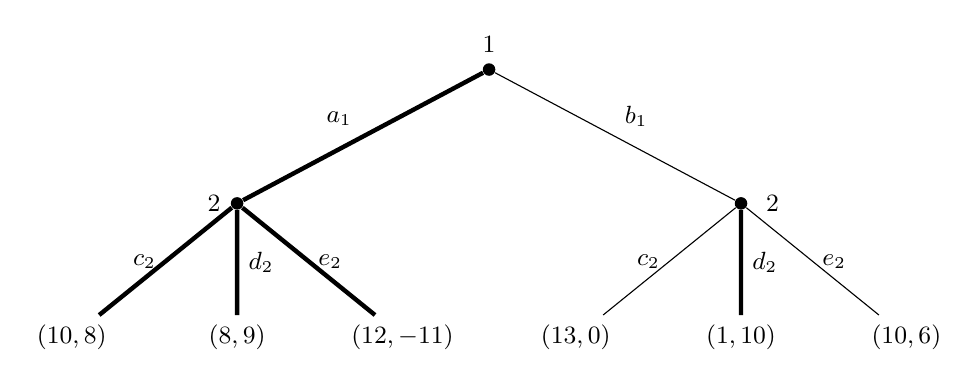
\begin{tikzpicture}[gametree,
  level 1/.style={sibling distance=64mm},
  level 2/.style={sibling distance=21mm}]
\node[dec,label=above:{1}] {}
  child { node[dec,label=left:{2\ }] {}
    child { node {$(10,8)$} edge from parent node[left] {$c_2$} }
    child { node {$(8,9)$} edge from parent[opt] node[right] {$d_2$} }
    child { node {$(12,-11)$} edge from parent node[right] {$e_2$} }
    edge from parent[opt] node[above left] {$a_1$} }
  child { node[dec,label=right:{\ 2}] {}
    child { node {$(13,0)$} edge from parent node[left] {$c_2$} }
    child { node {$(1,10)$} edge from parent[opt] node[right] {$d_2$} }
    child { node {$(10,6)$} edge from parent node[right] {$e_2$} }
    edge from parent node[above right] {$b_1$} };
\end{tikzpicture}
\end{center}
(Thick branches show the backward-induction choices; see 2.5.)

\subsection*{2.2 Strategy sets}
Player 1 moves once with 2 actions: $S_1=\{a_1,b_1\}$.

Player 2 has 2 information sets with 3 actions each, so she has $3\times3=9$ strategies. Write $xy$ for ``$x$ after $a_1$, $y$ after $b_1$'':
\[
S_2=\{c_2c_2,\ c_2d_2,\ c_2e_2,\ d_2c_2,\ d_2d_2,\ d_2e_2,\ e_2c_2,\ e_2d_2,\ e_2e_2\}.
\]
A common mistake is to write $S_2=\{c_2,d_2,e_2\}$. Those are Player 2's \emph{actions}. A strategy must say what she does after \emph{each} of Player 1's possible moves.

\subsection*{2.3 Building the normal form}
To fill the cell $(a_1, d_2e_2)$: Player 1 plays $a_1$, so Player 2 uses the \emph{first} entry of her plan, $d_2$. The outcome is $(a_1,d_2)$ and the payoffs are $(8,9)$. The second entry $e_2$ is \emph{off the path} and does not affect this cell, but it does affect the cells in the $b_1$ row. In general:
\[
u_i(a_1,xy)=u_i(a_1,x),\qquad u_i(b_1,xy)=u_i(b_1,y).
\]
That is why the $a_1$ row repeats in blocks of three ($x$ is constant within each block), while the $b_1$ row cycles ($y$ changes within each block).

\begin{center}
\small
\setlength{\tabcolsep}{4pt}
\begin{tabular}{r|ccccccccc}
 & $c_2c_2$ & $c_2d_2$ & $c_2e_2$ & $d_2c_2$ & $d_2d_2$ & $d_2e_2$ & $e_2c_2$ & $e_2d_2$ & $e_2e_2$ \\ \hline
$a_1$ & $10,8$ & $\underline{10},8$ & $\underline{10},8$ & $8,\underline{9}$ & $\underline{8},\underline{9}$ & $8,\underline{9}$ & $12,-11$ & $\underline{12},-11$ & $\underline{12},-11$ \\
$b_1$ & $\underline{13},0$ & $1,\underline{10}$ & $\underline{10},6$ & $\underline{13},0$ & $1,\underline{10}$ & $\underline{10},6$ & $\underline{13},0$ & $1,\underline{10}$ & $10,6$
\end{tabular}
\end{center}

\subsection*{2.4 All Nash equilibria}
\textbf{Underlining.} For Player 1, compare the two rows in each column (note the tie at $c_2e_2$: $10=10$). For Player 2, the maximum of the $a_1$ row is $9$, reached in the three columns starting with $d_2$; the maximum of the $b_1$ row is $10$, reached in the three columns ending with $d_2$. Only $(a_1,d_2d_2)$ has both payoffs underlined.

\textbf{The same thing as an argument} (this is what to write in an answer):
\begin{itemize}
\item If Player 1 plays $a_1$, Player 2's best responses are the plans with $d_2$ after $a_1$ (since $9>8>-11$), whatever she plans after $b_1$. For $a_1$ to be optimal, Player 1 must not prefer $b_1$, so $u_1(b_1,y)\le 8$. The candidates give $13$, $1$, and $10$, so only $y=d_2$ works, giving $(a_1,d_2d_2)$.
\item If Player 1 plays $b_1$, Player 2 needs $d_2$ after $b_1$. Then $b_1$ gives Player 1 only $1$, while $a_1$ gives $10$, $8$, or $12$. So there is no equilibrium with $b_1$.
\end{itemize}
\textbf{Answer:} the unique pure-strategy Nash equilibrium is $(a_1,d_2d_2)$, with outcome $(a_1,d_2)$ and payoffs $(8,9)$.

\textbf{Mixed equilibria (for full understanding).}
\begin{itemize}
\item Suppose Player 1 mixes with $\Pr(a_1)=p\in(0,1)$. Player 2's expected payoff from $xy$ is $p\,u_2(a_1,x)+(1-p)\,u_2(b_1,y)$, which separates into a part that depends only on $x$ and a part that depends only on $y$. So she picks the best $x$ and the best $y$ separately, which gives $d_2d_2$ uniquely. Against $d_2d_2$, $a_1$ gives $8>1$, so Player 1 won't mix. Contradiction.
\item With Player 1 playing $a_1$, Player 2 must play $d_2$ after $a_1$, but she is \emph{indifferent} about what to do after $b_1$, because that node is never reached. Let her randomize after $b_1$ with $(q_c,q_d,q_e)$. Player 1 stays with $a_1$ as long as
\[
13q_c+1\cdot q_d+10q_e\le 8 \iff 12q_c+9q_e\le 7 .
\]
So there is a whole family of mixed equilibria, all with the same outcome $(a_1,d_2)$.
\end{itemize}

\subsection*{2.5 Incredible threats?}
\textbf{Backward induction.} After $a_1$, Player 2 compares $8,9,-11$ and plays $d_2$. After $b_1$, she compares $0,10,6$ and plays $d_2$. Replace her nodes with the resulting payoffs: $a_1$ leads to $(8,9)$ and $b_1$ to $(1,10)$. Player 1 picks $a_1$ because $8>1$.
\[
\text{SPE}=(a_1,\ d_2d_2).
\]
\textbf{Answer: no.} The only pure Nash equilibrium is also the SPE. The threat that keeps Player 1 away from $b_1$ is ``I will play $d_2$ after $b_1$'', and Player 2 would really do that, because $d_2$ is her best reply in that subgame. A threat is incredible only if carrying it out would hurt the person making it. That is not the case here.

\textbf{Subtle point about the mixed family.} In those equilibria Player 2 puts weight on $c_2$ or $e_2$ after $b_1$, which is not optimal there, so they are not subgame perfect. But $c_2$ and $e_2$ would give Player 1 $13$ and $10$, which makes $b_1$ \emph{more} attractive. They act as promises, not threats, so nothing in those equilibria is held up by an incredible threat. Contrast this with Problem 5.

\begin{pitfall}
\begin{itemize}
\item Drawing a $2\times3$ matrix. That treats the game as simultaneous and ignores that Player 2 observes Player 1's move.
\item Reading Player 2's payoff from the wrong entry of her plan. In row $b_1$, use the \emph{second} letter.
\item Listing the equilibrium as the \emph{outcome} $(a_1,d_2)$. An equilibrium must give Player 2's \emph{whole} plan, $d_2d_2$.
\item Overlooking the $-11$. Getting its sign wrong changes Player 2's choice after $a_1$.
\end{itemize}
\end{pitfall}

\begin{selfcheck}
\begin{enumerate}
\item If $u_2(a_1,e_2)$ were $+11$, what would the SPE be, and would there be a non-subgame-perfect pure NE? \emph{(SPE $(a_1,e_2d_2)$. Also $(a_1,e_2e_2)$ is a NE, in which Player 2 plans $e_2$ after $b_1$ although $d_2$ is better there.)}
\item How many strategies would Player 2 have if Player 1 had 4 actions? \emph{($3^4=81$.)}
\end{enumerate}
\end{selfcheck}

%%%%%%%%%%%%%%%%%%%%%%%%%%%%%%%%%%%%%%%%%%%%%%%%%%%%%%%%%%%%%%%%%%%%%%%
\section{Timing and Strategies}

\textbf{What this tests:} the course notes' main warning that \emph{a strategy is not the same as an action}, and how timing and information change the normal form even when the physical actions stay the same (course notes, Example~3.3). The problem labels its parts 2.1--2.3; we keep those labels.

\subsection*{2.1 Simultaneous choice}
Player 2 does not see Player 1's choice, as in tree (a) of Section~0.2. Each player has one information set with actions $\{0,1\}$, so a strategy is simply ``pick 0'' or ``pick 1'':
\[
S_1=S_2=\{0,1\}.
\]
\begin{center}
\begin{tabular}{r|cc}
P1$\backslash$P2 & $0$ & $1$ \\ \hline
$0$ & $\underline{1},0$ & $0,\underline{1}$ \\
$1$ & $0,\underline{1}$ & $\underline{1},0$
\end{tabular}
\end{center}
No cell has both payoffs underlined, so there is no pure equilibrium. This is Matching Pennies with \$0/\$1 payoffs. \textbf{Mixed equilibrium.} Let $q=\Pr(\text{P2 plays }1)$. Player 1 gets $1-q$ from playing $0$ and $q$ from playing $1$; she is indifferent when $q=\tfrac12$. By symmetry, Player 2 is willing to mix only if $\Pr(\text{P1 plays }1)=\tfrac12$. So each player mixes $50/50$ and each expects $\$\tfrac12$. Each player's mixing keeps the \emph{opponent} indifferent.

\subsection*{2.2 Sequential choice}
Player 1 moves first, and Player 2 sees the move, as in tree (b). Player 1 still has $S_1=\{0,1\}$. Player 2 now has two information sets (``P1 chose 0'' and ``P1 chose 1''), so she has $2\times2=4$ strategies. Writing $(x,y)$ for ``$x$ after 0, $y$ after 1'':
\begin{center}
\begin{tabular}{cl}
$(0,0)$ & always play 0 \\
$(0,1)$ & copy Player 1 \\
$(1,0)$ & do the opposite of Player 1 \\
$(1,1)$ & always play 1
\end{tabular}
\end{center}

\subsection*{2.3 How the normal forms differ}
\begin{center}
\begin{tabular}{r|cccc}
P1$\backslash$P2 & $(0,0)$ & $(0,1)$ & $(1,0)$ & $(1,1)$ \\ \hline
$0$ & $\underline{1},0$ & $\underline{1},0$ & $\underline{0},\underline{1}$ & $0,\underline{1}$ \\
$1$ & $0,\underline{1}$ & $\underline{1},0$ & $\underline{0},\underline{1}$ & $\underline{1},0$
\end{tabular}
\end{center}
Points to make in your answer:
\begin{enumerate}
\item \textbf{Size.} The simultaneous game is $2\times2$; the sequential game is $2\times4$. The actions are the same, but Player 2 can condition on information, so she has more strategies.
\item \textbf{Where timing lives.} The normal form has no explicit timeline. Timing and information appear only through the strategy sets. You can see this in the repeated columns: $(0,0)$ and $(1,1)$ reproduce the simultaneous game's columns, while $(0,1)$ and $(1,0)$ are new plans that use information.
\item \textbf{Different predictions.} The strategy ``do the opposite'' $(1,0)$ gives Player 2 \$1 against \emph{any} Player 1 choice. Every equilibrium has Player 2 playing $(1,0)$, and Player 1 can play anything because she gets 0 either way. The pure equilibria are $(0,(1,0))$ and $(1,(1,0))$, with payoffs $(0,1)$. In the simultaneous game each player wins half the time. In this game moving second, with information, is an advantage.
\item \textbf{The normal form loses some detail.} The same $2\times4$ matrix also describes a simultaneous game in which Player 2 hands a referee a contingent plan ahead of time. The normal form cannot distinguish these two descriptions.
\end{enumerate}

\begin{pitfall}
\begin{itemize}
\item Saying Player 2's strategies in the sequential game are $\{0,1\}$. Those are her actions; her strategies are the four plans.
\item Saying the games have the ``same normal form because the payoffs are the same''. The payoff \emph{rules} are the same, but the strategy sets, and so the matrices, differ.
\end{itemize}
\end{pitfall}

%%%%%%%%%%%%%%%%%%%%%%%%%%%%%%%%%%%%%%%%%%%%%%%%%%%%%%%%%%%%%%%%%%%%%%%
\section{Third party observation of a game}

\textbf{What this tests:} the difference between \emph{money} and \emph{payoffs}, the definition of the normal form, constructing a game that rationalizes data, and what lab data can and cannot test. Parts are labelled 2.4--2.6 as in the prompt.

\subsection*{Step 0: reading the money table}
\begin{center}
\begin{tabular}{r|ccc}
 & $L_1$ & $M_1$ & $H_1$ \\ \hline
$L_2$ & \$8, \$8 & \$30, \$10 & \$15, \$1 \\
$M_2$ & \$10, \$30 & \$18, \$18 & \$20, \$4 \\
$H_2$ & \$1, \$15 & \$4, \$20 & \$5, \$5
\end{tabular}
\end{center}
Player 2 picks rows and Player 1 picks columns. The prompt does not say which dollar amount goes to whom. The game is symmetric, so it helps to write the money as ``\emph{my} \$ when I play $a$ and my opponent plays $b$''. The two possible readings give two different own-payoff tables:
\begin{center}
\begin{minipage}{0.46\textwidth}\centering
\textbf{Reading A}: first \$ = row player\\(the usual convention)\\[4pt]
\begin{tabular}{c|ccc}
mine $\backslash$ theirs & $L$ & $M$ & $H$ \\ \hline
$L$ & 8 & \underline{30} & 15 \\
$M$ & \underline{10} & 18 & \underline{20} \\
$H$ & 1 & 4 & 5
\end{tabular}
\end{minipage}
\hfill
\begin{minipage}{0.46\textwidth}\centering
\textbf{Reading B}: first \$ = Player 1\\(column player)\\[4pt]
\begin{tabular}{c|ccc}
mine $\backslash$ theirs & $L$ & $M$ & $H$ \\ \hline
$L$ & 8 & 10 & 1 \\
$M$ & \underline{30} & 18 & 4 \\
$H$ & 15 & \underline{20} & \underline{5}
\end{tabular}
\end{minipage}
\end{center}
(The underlined entry in each column is my best response to that opponent action.)

\textbf{Reading A} (a ``chicken''-type game). $H$ is strictly dominated by $M$: $10>1$, $18>4$, $20>5$. Between $L$ and $M$: against $L$ you want $M$, and against $M$ you want $L$. The pure equilibria are $(L_1,M_2)$ and $(M_1,L_2)$. There is also a mixed equilibrium: if the opponent plays $L$ with probability $q$, indifference requires $8q+30(1-q)=10q+18(1-q)$, so $q=6/7$.

\textbf{Reading B} (a social dilemma). $L$ is strictly dominated by $M$: $30>8$, $18>10$, $4>1$. Once $L$ is gone, $H$ strictly dominates $M$: $20>18$, $5>4$. The unique equilibrium is $(H_1,H_2)$ with \$5 each, even though $(M,M)$ would give both players \$18. This has the same structure as the Prisoner's Dilemma.

Under \emph{both} readings, $(M,M)$ is \emph{not} a Nash equilibrium of the money game. Against $M$, a player gains by switching to $L$ (Reading A: $30>18$) or to $H$ (Reading B: $20>18$). That is all we need for 2.4, and stating both readings protects your answer whichever convention the instructor intended.

\subsection*{2.4 Does universal $M$ reject a game-theoretic explanation?}
\textbf{Answer: no, not by itself.} The reasoning goes in three steps.
\begin{enumerate}
\item \emph{If} payoffs equal own money, then $(M_1,M_2)$ is not a Nash equilibrium, as shown above. Seeing every subject play $M$ is a systematic pattern, not random noise, so the data are inconsistent with ``players care only about their own money \emph{and} play a Nash equilibrium''.
\item But that is a \emph{joint} hypothesis. Game theory says players best-respond given their \emph{preferences}. The payoffs of a game are utilities over outcomes (Part 0.5), not dollar amounts. The experimenter controls the money but not how subjects value a pair of earnings such as (\$30, \$10) versus (\$18, \$18).
\item If subjects care about fairness, their partner's earnings, social norms, and so on, then they are playing a \emph{different game}: the same strategies but different payoffs. Universal $M$ can be the unique equilibrium of that game, as part 2.6 constructs.
\end{enumerate}
So what the data reject is the auxiliary assumption ``utility = own money'', not game theory.

\subsection*{2.5 The normal form, defined and explained}
Write the definition and explain each piece:
\begin{itemize}
\item $G=(N,\{S_i\},\{u_i\})$.
\item $N$: the players.
\item $S_i$: player $i$'s \emph{strategies}, that is, complete contingent plans that specify an action at every information set where $i$ moves, including ones that are never reached.
\item $u_i:S\to\mathbb{R}$: a \emph{utility representation} of $i$'s preferences over the outcomes that strategy profiles produce. It is ordinal for pure strategies and von Neumann--Morgenstern (unique up to positive affine transformations) once expected payoffs are used.
\end{itemize}
\textbf{Interpretation.} The normal form treats a game as if all players choose complete plans simultaneously and independently, and then the plans are carried out. It leaves out the timeline and the physical description. Timing and information survive only through what strategies can condition on (Problem 3). Applied here: $N=\{1,2\}$, $S_i=\{L_i,M_i,H_i\}$, and $u_i$ is \emph{how player $i$ values} each money pair, which is not necessarily her own dollars.

\subsection*{2.6 An explanation, and a game with unique NE $(M_1,M_2)$}
\textbf{The design goal.} The simplest way to get a \emph{unique} equilibrium is to make $M$ \emph{strictly dominant} for both players. Then IDSDS leaves only $(M,M)$, so it is the unique equilibrium, pure or mixed.

\textbf{A behavioral story.} $(M,M)$ is the only cell where both subjects earn a good \emph{and equal} amount (\$18 each). Every other high-earning cell is very unequal (\$30 vs.\ \$10, \$20 vs.\ \$4). Subjects who care about fairness and total earnings, and dislike leaving their partner badly off, will gravitate to $M$. A standard way to model this is \emph{social-welfare preferences} (Charness and Rabin, 2002): utility depends on total earnings and on the worse-off person's earnings. Take
\[
u_i(x_1,x_2)=x_1+x_2+\min\{x_1,x_2\}.
\]
(Equivalently $u_i=2\min\{x_1,x_2\}+\max\{x_1,x_2\}$: the worse-off person counts twice.)

\textbf{Why this choice is convenient.} The formula is symmetric in $(x_1,x_2)$, so both players have the \emph{same} utility in every cell, and it does not matter which dollar amount goes to whom. The Reading A/B issue disappears. Cell by cell:
\[
(8,8)\mapsto 24,\quad (30,10)\mapsto 50,\quad (15,1)\mapsto 17,\quad (18,18)\mapsto 54,\quad (20,4)\mapsto 28,\quad (5,5)\mapsto 15.
\]
\begin{center}
\begin{tabular}{r|ccc}
 & $L_1$ & $M_1$ & $H_1$ \\ \hline
$L_2$ & $24,24$ & $\underline{50},\underline{50}$ & $17,17$ \\
$M_2$ & $\underline{50},\underline{50}$ & $\underline{54},\underline{54}$ & $\underline{28},\underline{28}$ \\
$H_2$ & $17,17$ & $\underline{28},\underline{28}$ & $15,15$
\end{tabular}
\end{center}
\textbf{Verify dominance.} For the row player, row $M$ is $(50,54,28)$, row $L$ is $(24,50,17)$, and row $H$ is $(17,28,15)$. $M$ is strictly larger in every column, and the same holds for the column player by symmetry. So $M$ is strictly dominant for both players and $(M_1,M_2)$ is the unique Nash equilibrium.

\textbf{Other stories that also work} (if you want to propose a different one):
\begin{itemize}
\item \emph{Norm-following.} Subjects feel a psychological cost $c$ from not picking the ``fair'' middle option: $u_i=\text{own }\$-c\cdot\mathbf{1}\{a_i\ne M\}$. Check that $c>12$ makes $M$ strictly dominant under both readings. (The binding comparison is $18>30-c$ in Reading A.)
\item \emph{Inequity aversion} (Fehr and Schmidt, 1999): $u_i=x_i-\alpha\max\{x_j-x_i,0\}-\beta\max\{x_i-x_j,0\}$. Be careful: under Reading B, $(H,H)$ stays an equilibrium for any $\alpha,\beta\ge 0$, because $(5,5)$ is already equal. So this story gives multiple equilibria there, not a unique one. Always verify uniqueness.
\end{itemize}

\subsection*{Can experiment data like this test rationality?}
\textbf{Answer: not by themselves.}
\begin{itemize}
\item \emph{Rational} means maximizing \emph{some} complete, transitive preference given one's beliefs. Choices in one game can be explained by many different preferences, and the experimenter observes only money and choices, not utility.
\item Part 2.6 shows the problem concretely: \emph{whatever} profile we observe, we can make it the unique, even dominant-strategy, equilibrium by choosing the preferences. A hypothesis that can explain any data cannot be refuted by those data.
\item What the experiment \emph{can} test is a \emph{joint} hypothesis: rationality plus a specific utility function (for example, ``own money only'') plus equilibrium beliefs. Here that joint hypothesis is rejected.
\item To learn about rationality itself you need restrictions that tie preferences together across situations. Examples: run many games with different payoffs and check whether a single stable utility function rationalizes all the choices (a revealed-preference/consistency test, as in Chapter 1); elicit beliefs separately; include one-person decision problems with the same money outcomes so that strategic uncertainty is removed.
\end{itemize}

\begin{pitfall}
\begin{itemize}
\item Answering 2.4 with ``yes, $(M,M)$ isn't a NE, so game theory is rejected''. That treats the money table as the game.
\item In 2.6, writing a matrix where $(M,M)$ is \emph{a} NE but not the \emph{unique} one. Check every cell, or use strict dominance.
\item Claiming the data ``prove players are irrational''. Without knowing their preferences you cannot conclude that.
\end{itemize}
\end{pitfall}

%%%%%%%%%%%%%%%%%%%%%%%%%%%%%%%%%%%%%%%%%%%%%%%%%%%%%%%%%%%%%%%%%%%%%%%
\section{Subgame Perfect Nash Equilibrium}

\textbf{What this tests:} the whole pipeline (tree, normal form, NE, SPE) and seeing an incredible threat at work. The prompt says Player 1 moves again ``after observing player 2's action''. That is a typo: the subscripts make clear that \textbf{Player 2} observes Player 1's choice and then picks $U_2$ or $D_2$. Say so in your answer.

\subsection*{5.1 Normal form}
$N=\{1,2\}$ and $S_1=\{L_1,M_1,H_1\}$. Player 2 has 3 information sets (one after each Player 1 action) with 2 actions each, so she has $2^3=8$ strategies. Write $x_Lx_Mx_H$, where $x_k\in\{U_2,D_2\}$ is what she does after $k_1$:
\[
S_2=\{UUU,UUD,UDU,UDD,DUU,DUD,DDU,DDD\}.
\]
Payoffs: $u_i(k_1,\ x_Lx_Mx_H)=u_i(k_1,x_k)$. Player 1's choice determines which letter of Player 2's plan is used.

\subsection*{5.2 Matrix and all Nash equilibria}
How to fill row $M_1$: use the \emph{middle} letter. Column $DUD$ has middle letter $U$, so the cell is $u(M_1,U_2)=(5,5)$.
\begin{center}
\small
\setlength{\tabcolsep}{4pt}
\begin{tabular}{r|cccccccc}
 & $UUU$ & $UUD$ & $UDU$ & $UDD$ & $DUU$ & $DUD$ & $DDU$ & $DDD$ \\ \hline
$L_1$ & $\underline{10},10$ & $\underline{10},10$ & $\underline{10},10$ & $\underline{10},10$ & $1,\underline{11}$ & $1,\underline{11}$ & $1,\underline{11}$ & $1,\underline{11}$ \\
$M_1$ & $5,5$ & $5,5$ & $2,\underline{6}$ & $2,\underline{6}$ & $\underline{5},5$ & $\underline{5},5$ & $\underline{2},\underline{6}$ & $2,\underline{6}$ \\
$H_1$ & $1,4$ & $3,\underline{5}$ & $1,4$ & $3,\underline{5}$ & $1,4$ & $3,\underline{5}$ & $1,4$ & $\underline{3},\underline{5}$
\end{tabular}
\end{center}
Two cells have both payoffs underlined: $(M_1,DDU)$ and $(H_1,DDD)$.

\textbf{The same result by reasoning} (the cleaner write-up). Player 2 strictly prefers $D_2$ after every action ($11>10$, $6>5$, $5>4$), so in any equilibrium she plays $D_2$ at the node that is \emph{reached}. Off the path she is free, and those off-path choices are what determine which Player 1 actions are deterred.
\begin{itemize}
\item \emph{Can $L_1$ be played?} Player 2 must answer $D_2$, so Player 1 gets 1. But $M_1$ always gives Player 1 at least 2. So no.
\item \emph{$M_1$:} Player 2 plays $D_2$ after $M_1$, and Player 1 gets 2. To keep Player 1 from deviating: after $L_1$ she needs $D_2$ (otherwise $L_1$ gives 10), and after $H_1$ she needs $U_2$ (otherwise $H_1$ gives 3). This gives $(M_1,DDU)$.
\item \emph{$H_1$:} Player 2 plays $D_2$ after $H_1$, and Player 1 gets 3. She needs $D_2$ after $L_1$ (else 10) and $D_2$ after $M_1$ (else 5). This gives $(H_1,DDD)$.
\end{itemize}
\textbf{Answer:} the pure Nash equilibria are $(M_1,D_2D_2U_2)$ with payoffs $(2,6)$ and $(H_1,D_2D_2D_2)$ with payoffs $(3,5)$.

\textbf{Mixed versions.} Player 1 never mixes: if she mixed over two actions, Player 2 would play $D_2$ at both, and Player 1's payoffs from them ($1,2,3$) differ, so she would not be indifferent. Player 2 can mix \emph{off the path}:
\begin{itemize}
\item Outcome $(M_1,D_2)$: need $1+9\Pr(U\mid L)\le 2$ and $3-2\Pr(U\mid H)\le 2$, i.e.\ $\Pr(U\mid L)\le\tfrac19$ and $\Pr(U\mid H)\ge\tfrac12$.
\item Outcome $(H_1,D_2)$: need $1+9\Pr(U\mid L)\le 3$ and $2+3\Pr(U\mid M)\le 3$, i.e.\ $\Pr(U\mid L)\le\tfrac29$ and $\Pr(U\mid M)\le\tfrac13$.
\end{itemize}

\subsection*{5.3 Game tree and SPE}
\begin{center}
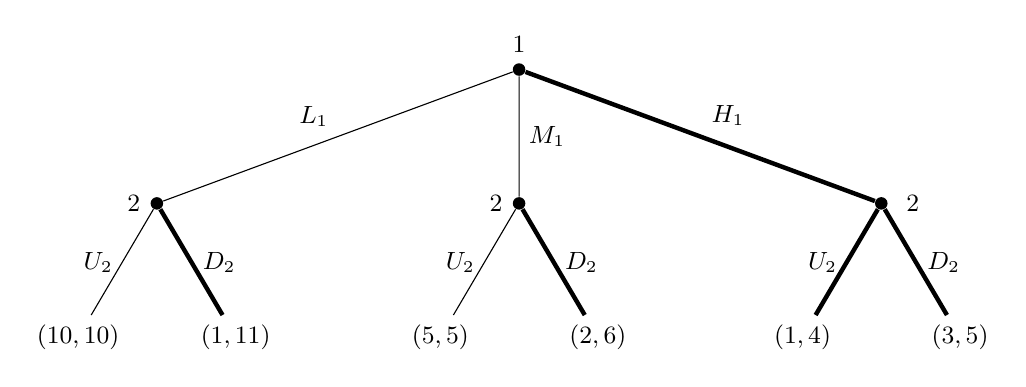
\begin{tikzpicture}[gametree,
  level 1/.style={sibling distance=46mm},
  level 2/.style={sibling distance=20mm}]
\node[dec,label=above:{1}] {}
  child { node[dec,label=left:{2\ }] {}
    child { node {$(10,10)$} edge from parent node[left] {$U_2$} }
    child { node {$(1,11)$} edge from parent[opt] node[right] {$D_2$} }
    edge from parent node[above left] {$L_1$} }
  child { node[dec,label=left:{2\ }] {}
    child { node {$(5,5)$} edge from parent node[left] {$U_2$} }
    child { node {$(2,6)$} edge from parent[opt] node[right] {$D_2$} }
    edge from parent node[right] {$M_1$} }
  child { node[dec,label=right:{\ 2}] {}
    child { node {$(1,4)$} edge from parent node[left] {$U_2$} }
    child { node {$(3,5)$} edge from parent[opt] node[right] {$D_2$} }
    edge from parent[opt] node[above right] {$H_1$} };
\end{tikzpicture}
\end{center}
\textbf{Backward induction.}
\begin{enumerate}
\item \emph{Last movers.} After $L_1$: $11>10$, so $D_2$. After $M_1$: $6>5$, so $D_2$. After $H_1$: $5>4$, so $D_2$.
\item \emph{Reduced game for Player 1.} $L_1$ leads to $(1,11)$, $M_1$ to $(2,6)$, and $H_1$ to $(3,5)$. She picks $H_1$.
\end{enumerate}
\textbf{Answer:} the unique SPE is $(H_1,\ D_2D_2D_2)$, with outcome $(H_1,D_2)$ and payoffs $(3,5)$.

\textbf{The incredible threat, explained.} In the other Nash equilibrium $(M_1,DDU)$, Player 2 effectively says: ``If you play $H_1$, I'll play $U_2$ and you'll get only 1.'' That keeps Player 1 at $M_1$, which is better for Player 2 ($6>5$). But if Player 1 actually played $H_1$, Player 2 would compare $U_2$ (4) with $D_2$ (5) and play $D_2$. The threat would not be carried out, Player 1 can see this, and so the equilibrium falls apart. Nash equilibrium does not catch this, because the threat is never tested: the node after $H_1$ is never reached, and changing an action at an unreached node does not change Player 2's payoff. Subgame perfection catches it by requiring optimal play in \emph{every} subgame.

\textbf{Comparison with Problem 2.} In Problem 2 the deterring action ($d_2$ after $b_1$) was Player 2's genuine best reply, so the threat was credible and the Nash equilibrium was the SPE. Here the deterring action ($U_2$ after $H_1$) is not her best reply, so the threat is incredible and the Nash equilibrium is not an SPE.

\begin{pitfall}
\begin{itemize}
\item Following the typo literally and having Player 1 move twice.
\item Stating the SPE as $(H_1,D_2)$. That is the \emph{outcome}. The SPE must list Player 2's action at all three nodes: $D_2D_2D_2$.
\item Missing $(M_1,DDU)$ because ``Player 2 always plays $D$''. Off-path choices are unconstrained by Nash equilibrium, so you must check them.
\end{itemize}
\end{pitfall}

\begin{selfcheck}
\begin{enumerate}
\item Why is $(M_1,DDD)$ not a NE? \emph{(Player 1 would switch to $H_1$: $3>2$.)}
\item Why is $(H_1,DUD)$ not a NE? \emph{(Player 1 would switch to $M_1$: $5>3$.)}
\item Which NE does Player 2 prefer, and why can't she get it in an SPE? \emph{($(M_1,DDU)$ gives her 6. She would need to commit to $U_2$ after $H_1$, and that commitment is not credible.)}
\end{enumerate}
\end{selfcheck}

%%%%%%%%%%%%%%%%%%%%%%%%%%%%%%%%%%%%%%%%%%%%%%%%%%%%%%%%%%%%%%%%%%%%%%%
\section*{Cheat sheet}
\addcontentsline{toc}{section}{Cheat sheet}
\begin{center}
\renewcommand{\arraystretch}{1.25}
\begin{tabular}{p{0.28\textwidth}p{0.64\textwidth}}
\hline
\textbf{Concept} & \textbf{One-line test} \\ \hline
Strategy & An action at \emph{every} information set; $|S_i|=\prod_h(\#\text{actions at }h)$. \\
Strictly dominated & Strictly worse than some other strategy against \emph{every} opponent strategy. \\
IDSDS & Delete strictly dominated strategies, repeat on the smaller game; order doesn't matter. \\
Nash equilibrium & Every player is best-responding; no profitable unilateral deviation. \\
Finding pure NE & Underline best responses; cells with both payoffs underlined. \\
Mixed NE & Each player's probabilities make the \emph{other} indifferent over her support. \\
IDSDS $\leftrightarrow$ NE & Deleted strategies never appear in any NE; a unique survivor is the unique NE. \\
SPE & NE in every subgame; found by backward induction; list choices at every node. \\
Incredible threat & An off-path action the player would not choose if that node were reached. \\
Payoffs & Utilities over outcomes, not money; experiments control money, not preferences. \\ \hline
\end{tabular}
\end{center}

\end{document}
